% Created 2020-02-13 Thu 17:18
% Intended LaTeX compiler: xelatex
\documentclass[11pt]{article}
\usepackage{graphicx}
\usepackage{grffile}
\usepackage{longtable}
\usepackage{wrapfig}
\usepackage{rotating}
\usepackage[normalem]{ulem}
\usepackage{amsmath}
\usepackage{textcomp}
\usepackage{amssymb}
\usepackage{capt-of}
\usepackage{hyperref}
\usepackage{fontspec}
\usepackage{CJK}
\usepackage{ctex}
\usepackage{geometry}
\usepackage{xcolor}
\usepackage[hidelinks]{hyperref}
\usepackage[bibstyle=gb7714-2015,
citestyle=gb7714-2015,
backend=biber,
backref=true,
seconds=true,
sorting=none]{biblatex}
\addbibresource{../main.bib}
\newCJKfontfamily[fsong]\myfsong{FangSong}
\newCJKfontfamily[fhei]\myheiti{SimHei}
\newCJKfontfamily[fzxiaobiao]\myfzxiaobiao{方正小标宋_GBK}
\newCJKfontfamily[ftimes]\mytimes{Times New Roman}
\setCJKmainfont[AutoFakeBold]{SimSun}
\setCJKsansfont[AutoFakeBold]{SimHei}
\setmainfont{Times New Roman}
\setsansfont{Arial}
\geometry{
paper      = a4paper,
vmargin    = 2.54cm,
left       = 2.5cm,
right      = 2cm,
headheight = 0.75cm,
headsep    = 0.29cm,
footskip   = 0.79cm,
}
\hypersetup{
colorlinks=true,
pdfstartview=FitH,
linkcolor={blue!50!black},
anchorcolor=violet,
citecolor=magenta}
\author{hexinzheng}
\date{\today}
\title{EMACS NOTES}
\hypersetup{
 pdfauthor={hexinzheng},
 pdftitle={EMACS NOTES},
 pdfkeywords={},
 pdfsubject={},
 pdfcreator={Emacs 26.1 (Org mode 9.2.6)}, 
 pdflang={English}}
\begin{document}

\maketitle
\tableofcontents


\section{问题}
\label{sec:org08994bd}
\begin{itemize}
\item[{$\boxminus$}] org 转换为标准 latex 文件
\item[{$\boxminus$}] org 输出为 html 文件
\item[{$\boxminus$}] 使用 github 样式显示文件
\item[{$\boxtimes$}] 在 github 上建立自己的站点
\item[{$\boxtimes$}] 默认浏览器改为 qutebrowser
\item[{$\boxminus$}] 安装 emacs 26.1 。主要是 emacs-26-non-common-dfsg.
\item[{$\boxminus$}] Open org-mode html in EWW.
\end{itemize}

\section{调试脚本}
\label{sec:org293d7f2}
\begin{itemize}
\item 单独加载另外一个 emacs 的初始化文件
\end{itemize}
\begin{verbatim}
emacs -q -l ~/youemacs.el
emacs --no-initial-file --load-file=~/youemacs.el
\end{verbatim}

\begin{itemize}
\item 调试 elisp 语言, , '  ,或是 M-x
 ielm 。
\end{itemize}

\section{澄清概念}
\label{sec:orgca268f0}
\begin{enumerate}
\item 组合键的术语是 Command, 而不是 ShortCut
\label{sec:org4c8b3e9}
例如,搜索插入文件变量的组合键,关键词应为 \uline{command file variable emacs}
。如使用 \uline{shortcut \ldots{}} 则无法找到有用结果。
\end{enumerate}
\section{重要概念}
\label{sec:orgc8d7eb7}
\subsection{屏幕(Screen)}
\label{sec:org10cb301}
Emacs 的显示区域称为 Frame , 在 Frame 中可包含多个 Windows。 Emacs 中 Frame 在 IDE 中称为 Windows, 而 Emacs 的 Windows 在 IDE 中称为 View。
\subsubsection{Point}
\label{sec:orged5c737}
称为输入提示符号。通过 Cursor 可以改变输入符号的显示。
\subsubsection{Echo Area}
\label{sec:org3ddf384}
显示输入命令的区域。Display Custom 修改 Echo Area。Echo Area 用于显示 Minibuffer。退出 Minibuffer 命令是 C-g。
\subsubsection{Mode Line}
\label{sec:orgd383495}
窗口底部是 Mode Line,显示当前 buffer 状态。Mode Line 文本格式如下

\begin{center}
\begin{tabular}{lllllll}
cs & ch-fr & buf & pos & line & (major & minor)\\
\end{tabular}
\end{center}

以下是详细解释

\begin{center}
\begin{tabular}{ll}
cs & Coding System 的缩写。C-h C unix 给出 unix coding 的具体信息。 C-h C uft-8 给出 utf-8 coding 的具体信息。\\
ch & 表示文件是否保存。 * 表示文件未保存, - 表示文件已保存,\% 表示为只读文件。\\
fr & Frame 缩写。 F1 为第 1 个 Frame,F2 为第 2 个 Frame。\\
buf & Buffer name,即当前 Buffer 中文件名。\\
pos & 当前 Buffer 中显示的文件位置。 Top 靠近文件首部, Bot 靠近文件尾部, All 显示了全部文件,nn\% 以百分比形式指出显示位置。\\
line & 18:10 表示 第 18 行第 10 个字符位置。\\
major & 主编辑模式,如 Text mode,Lisp mode,Latex mode 等。\\
minor & 次编辑模式,可附加到主编辑模式之后。\\
recursive edit & [\ldots{}] 表示处于循环编辑模式。\\
\end{tabular}
\end{center}

\subsection{用户输入(User input)}
\label{sec:org2d9df71}
Emacs 主要设计目的是通过键盘与用户交互,当然 Emacs 也使用鼠标,但这不是设计的出发点。 因而要能熟练使用键盘快捷键操作和编辑文件。
\subsection{输入键 (Keys)}
\label{sec:orgb423bf0}
Key 和其组合键会引发 key event。如果一组 Key 引发一条命令,称为 Complete Key。 如果无法触发命令,称为 Prefix key,如 C-x 和 M-x。
\subsection{命令 (Command)}
\label{sec:org1339067}
每条命令是一个 Lisp 函数。 将命令与组合键绑定在一起称为 Keymaps。 C-n 之所以能跳到下一行,是因为绑定了函数 next-line。
\subsection{进入 Emacs}
\label{sec:orgb1fa037}
如果 inhibit-startup-screen 为 non-nil 将不会显示欢迎界面,而直接进入到 \textbf{scratch} 文件,在其中能运行一些待测试的 Lisp 程序。

如果希望启动 Emacs 时,进入到某个目录或是打开特定文件,可配置 initial-buffer-choice 。
\subsection{退出 Emacs}
\label{sec:org69b860e}
C-x C-x 退出 Emacs (save-buffers-kill-terminal)
C-z     Emacs 最小化 (suspend-frame)
M-x kill-emacs 退出 Emacs,不需要任何提示

Emacs 能在退出时保存当前会话 Session,下次启动后可先加载此会话。
\section{基本编辑命令}
\label{sec:org4ce4dca}
\subsection{基础}
\label{sec:org78c10d1}
\subsubsection{插入文本 (Insert Text)}
\label{sec:org1a46690}
\texttt{C-j} [O] 插入新的空行,新行没有 auto-indent 。 在 Minor Mode 中, 可以改变插入方式。 例如, \texttt{Auto Fill Mode} 可自动截取超出长度的文本(参见 Filling)。

如要插入非图形化字符,先输入 \texttt{C-q} (quoted-insert)
\begin{itemize}
\item 输入 DEL 。 \texttt{C-q} 后,紧接着输入 <DEL>。
\item 输入 Unicode。 \texttt{C-q 1 0 1 B} 显示 AB。
\end{itemize}

\texttt{read-quoted-char-radix} 控制基数,如果为 10 表示十进制,如果为 16 表示十六进制。

Unicode 字符还可以通过 \texttt{C-x 8} 命令插入, \texttt{C-x 8 C-h} 查看具体插入 Unicode 字符的命令。 例如, \texttt{C-x 8 \$} 插入字符  ¤ 。
或者 \texttt{C-x 8 <RET>} 会列出所有 Unicode 可用字符。 例如,输入 lambda ,找到对应命令 \texttt{Greek Small Letter Lambda} 就能插入 λ 。

\subsubsection{移动光标 (Move Point)}
\label{sec:org9101324}
我使用 Evil-mode 所以不太用这些操作。

\subsubsection{删除 (Erasing)}
\label{sec:orgf6ceed7}
\begin{center}
\begin{tabular}{lll}
Emacs & Function & Evil\\
\hline
<DEL> & delete-forward-char & x\\
<BACKSPACE> & delete-backward-char & X\\
\texttt{C-d} & delete-char & x\\
\texttt{C-k} & kill-line & dd\\
\texttt{M-d} & kill-word & D\\
\end{tabular}
\end{center}

\subsubsection{基本撤销 (Basic Undo)}
\label{sec:orgf419e0b}

\begin{center}
\begin{tabular}{lll}
Emacs & Function & Evil\\
\texttt{C-x u} & undo & u\\
\texttt{M-x \_} & redo & \\
\end{tabular}
\end{center}
\subsubsection{文件 (Files)}
\label{sec:org0049ef8}

\begin{center}
\begin{tabular}{lll}
Emacs & Function & Evil\\
\texttt{C-x C-f} & find-file & \\
\texttt{C-x C-s} & save-buffer & \\
\end{tabular}
\end{center}

\subsubsection{帮助 (Help)}
\label{sec:org161d4a8}
简单,直接 \texttt{C-h} 即可。

\subsubsection{空行 (Blank Lines)}
\label{sec:org3f50bb3}

\begin{center}
\begin{tabular}{lll}
Emacs & Function & Evil\\
\texttt{C-x C-o} & delete-blank-lines & 类似 J\\
\texttt{C-o} & open-line & o\\
\end{tabular}
\end{center}

\subsubsection{连续行 (Continuation Lines)}
\label{sec:orga819494}

:ID:       0500a5b8-4fdb-4b52-9beb-472db7ab2bda

在新版 org-mode (>9.0) 中, 不再使用 \texttt{<s tab} 插入代码。Easy template 换为了 \texttt{C-c C-,} 。

在 org-mode 中,插入按键顺序的命令 SPC m i k  。

\begin{figure}[htbp]
\centering
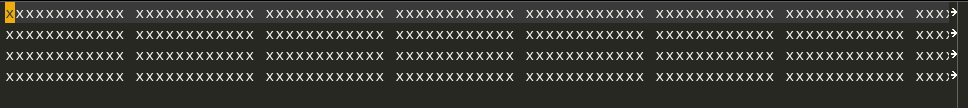
\includegraphics[width=.9\linewidth]{./pic/trunc1.png}
\caption{\label{fig:org3ef2972}
使用 SPC t l  启用 line truncation}
\end{figure}

\subsubsection{位置信息 (Position Info)}
\label{sec:org17d0479}
\subsubsection{参数 (Arguments)}
\label{sec:orga5288aa}
\subsubsection{重复 (Repeating)}
\label{sec:orgfe9150c}
\subsection{Minibuffer}
\label{sec:org99244bd}
\subsection{M-x}
\label{sec:org2aa48cf}
\subsection{帮助(help)}
\label{sec:orgd0e1bef}
\section{org-mode}
\label{sec:org941acfc}
\subsection{Agenda Views}
\label{sec:orgcf4da56}
Todo items 、 time-stamped items 和 tagged headlines 可能分布在不同的文件中。
有时为了能将这些信息搜集、整理并按照要求提取信息,在特定 buffer 中显示,这种
方式称为 Agenda。
\subsubsection{Agenda Files}
\label{sec:orge66a857}
\texttt{org-agenda-files} 存放 agenda 文件指定位置,通常是配置为目录,该目录下所
有 .org 文件都是 agenda 文件。 如果只有一个 agenda 文件就必须明确给出文件名。
\begin{verbatim}
(setq org-agenda-files (list "~/gitdown/MyThrougth/mytime.org"))
\end{verbatim}

因此 agenda 是由一组 org 文件构成的,依次读取每个文件内容,搜集文件信息。
比较便捷的方式是直接用命令 C-c [  把当前文件
添加到 agenda 中 , C-c ]  已修改为在当前文件
中插入 Bibtex 引用。因此,要使用 org-remove-file 命令直接从 agenda 文件中
移除当前 org 文件。 C-c ,  循环访问 agenda 文件。

\subsection{Document Structure}
\label{sec:org34a7cb1}
\subsubsection{Headlines}
\label{sec:orgd242402}
\begin{center}
\begin{tabular}{ll}
local visible cycling &  <tab> \\
global visible cycling &  <backtab> \\
move up/down &  <M-up>  / <M-down> \\
\end{tabular}
\end{center}
\subsection{ToDo Items}
\label{sec:org3e14dd5}
\begin{enumerate}
\item Basic
\label{sec:orgbc23250}
\end{enumerate}
\subsection{Datetimes}
\label{sec:orgfbbb835}
ToDo items 可以标记 date 和 time, 在 org 中称之为 timestamp。
\subsubsection{Timestamps}
\label{sec:orge1f50c4}
时间戳分类
\begin{enumerate}
\item 普通时间戳;事件;约会
\label{sec:org5dd70b4}
只分配 date/time 形式的时间戳,在显示 agenda 时,只显示 date。
\begin{enumerate}
\item 周六看电影\textit{<2019-11-30 Sat>}
\label{sec:org758b120}
\item 周四吃晚餐\textit{<2019-11-28 Thu>}
\label{sec:org838bb14}
\end{enumerate}
\item 规律重复出现的时间戳
\label{sec:org991dcc3}
如每天下午 5 点跑步,每周六去公园玩,每年的生日等。
\textbf{d} 表示 day, \textbf{w} 表示 week , \textbf{m} 表示 month。
\item 用 sexp 表示复杂日期
\label{sec:org33f1c24}
牵涉到 LISP 语言中的 S-exp 表达式,暂不考虑。可以用来安排课程表。 
\item 指定 Time/Date 范围
\label{sec:orgd15d1e1}
由 \texttt{-{}-} 连接的两个日期表示范围。
\begin{enumerate}
\item 论文答辩\textit{<2019-12-10 Tue>--<2019-12-13 Fri>}
\label{sec:org96fae37}
\end{enumerate}
\item 非激活日期
\label{sec:orgc8b0932}
由 \texttt{[ ]} 包含的日期,并不会出现在 agenda 中。
\begin{enumerate}
\item 和朋友聚餐 \textit{[2019-11-28 Thu]}
\label{sec:org978eb85}
\end{enumerate}
\end{enumerate}
\subsubsection{创建时间戳}
\label{sec:org8e2f141}
\begin{center}
\begin{tabular}{ll}
 C-c .  & 插入日期/连续日期\\
 C-c !  & 插入非激活日期\\
 C-c <  & 插入当前日期\\
 C-c C-o  & 列出光标下日期/日期范围中的 agenda\\
 <S-right>  <S-left>  & 调整月份\\
 <S-up>  <S-down>  & 调整天数\\
 C-c C-y  & 计算有多少天\\
\end{tabular}
\end{center}
\subsubsection{Deadlines 和 Scheduling}
\label{sec:orgbac4ab2}
时间戳可配置特殊关键字帮助进行计划,例如 Deadlines 和 Scheduling。

使用 C-c /   会出现 sparse tree。

\begin{enumerate}
\item DEADLINE
\label{sec:org282c824}
所有 DEADLINE 日期之前计划的事件都会显示在 agenda 中,
\texttt{org-deadline-warning-days} 指定 DEADLINE 日期之前几天发出警告,直到将事
件标志为 DONE 才会停止提示警告。
\begin{enumerate}
\item 完成课程教案编写工作
\label{sec:org29cbc98}
\begin{verbatim}
DEADLINE:<2019-11-30 Sat>
第一次编辑:[[bbdb:Ford Prefect]]
\end{verbatim}

使用 \texttt{-2d} 表示提前 2 天发出警告提示。
\item 与张总见面约谈
\label{sec:org1371691}
\begin{verbatim}
DEADLINE:<2019-11-30 Sat -2d> 
\end{verbatim}

重复某个 Deadlines,使用 \texttt{+1m} 表示每月重复一次,\textasciitilde{}-2d\textasciitilde{} 表示提前 2 天提示。
当本月任务完成后,再次使用 C-c C-t  不但能
标记本月任务已经完成,而且还能启用下月任务。 凡是标记为 DONE 的任务不再
出现在 agenda 中。
\item 交房租
\label{sec:org0ce5b37}
\begin{verbatim}
DEADLINE: <2019-08-15 Thu +1m -2d>
:PROPERTIES:
:LAST_REPEAT: [2019-11-28 Thu 15:27]
:END:
\end{verbatim}

\item 与 Scott 老师视频通话
\label{sec:org2bf4ee8}
\begin{verbatim}
SCHEDULED: <2019-10-25 Fri ++1w>
:PROPERTIES:
:LAST_REPEAT: [2019-11-28 Thu 15:26]
:END:
\end{verbatim}
\end{enumerate}
\item SCHEDULED
\label{sec:org0f5ec51}
计划何时开始某项新任务。如果延迟两天才开始该任务,则显示为 \texttt{2x} 。如果计
划推迟 3 天,则在时间上使用 \texttt{-3d} 表示。

SCHEDULED 经常会被误解。 例如,与某人约会是 appointment,使用简单的计划即
可。 一旦使用 SCHEDULED , 则表示在该任务在指定日期才会在时间线中出现。
\begin{enumerate}
\item 去新加坡旅行
\label{sec:org31f1bd2}
\begin{verbatim}
SCHEDULED:<2019-11-24 Sun --2d> 
\end{verbatim}
\end{enumerate}
\end{enumerate}

\section{Timer Example}
\label{sec:orgaeb64cd}

\subsection{Clock column view example}
\label{sec:orgb9baf0d}

\subsection{Effort estimate example}
\label{sec:orga4c27ca}

\section{Orgmode (Studing)}
\label{sec:orge7ac046}
\subsection{E01S01 : Headlines \& outline mode}
\label{sec:org02435ca}
\noindent\textbf{CLOSED:} \textit{[2020-02-10 Mon 21:25]}\\
\begin{center}
\begin{tabular}{ll}
Local expand/collapse cycle &  <tab> \\
Global expand/collapse cycle &  <backtab> \\
Increase level &  <alt-right> \\
Decrease level &  <alt-left> \\
Move up &  <M-up> \\
Move down &  <M-down> \\
\end{tabular}
\end{center}

\subsection{E01S03 : Schedule, Deadlines \& Agenda views}
\label{sec:org7f0411c}
\begin{center}
\begin{tabular}{ll}
Schedule done &  C-c C-s \\
Deadlines defined &  C-c C-d \\
Agenda switch &  C-a a \\
Follow mode &  S-f \\
Move forward &  f \\
Move backward &  b \\
\end{tabular}
\end{center}
\subsection{E01S04 : Repeating tasks}
\label{sec:orgcc5daf8}
\begin{center}
\begin{tabular}{ll}
regular every week (d=day w=weak m=month y=year) & +1w\\
repeat every week, definitely in the future & ++1w\\
Next 4 week after the task is DONE & .+4w\\
\end{tabular}
\end{center}

If repeated event was setting by SCHEDULED  C-c C-t
 , you could press  C-c C-t 
again to change current SCHEDULED event to state DONE and restart a new
SCHEDULED event.

\subsubsection{规律重复出现的时间戳}
\label{sec:orgf5bfde5}
如每天下午 5 点跑步,每周六去公园玩,每年的生日等。
\textbf{d} 表示 day, \textbf{w} 表示 week , \textbf{m} 表示 month。
\subsection{E01S05 : Checklists [2/4]}
\label{sec:org0636fd6}
\begin{itemize}
\item[{$\square$}] This is checklist
\item[{$\square$}] New checklist by  <M-S-return>
\item[{$\boxtimes$}] You can see the completion of the checklist with [0/0] or [0\%] on headlines.
\item[{$\boxtimes$}] Checkbox toggled with  C-c C-c
\end{itemize}
\subsection{E02S01 : Tags}
\label{sec:orgca57c70}
Tags can be added to headlines and are often used as a way to mark GTD contexts.

Tags can be predefined with a line \texttt{\#+TAGS:PHONE(o) ...} at the beginning of
the file. Use  C-c C-q  to assign a tags for a
headline. Use  <tab>  to enter new tags instead
of predefined tags. Clear tags by  SPC  .

\subsection{E02S02 : Agenda view (advanced)}
\label{sec:orgb8fa89c}
\begin{center}
\begin{tabular}{ll}
Timeline for current buffer &  L \\
List all TODO entries &  t \\
Entries with a special TODO Keywords &  T \\
Match tags/propoerties/TODO keywords &  M \\
Like before, but only TODO keywords &  M \\
Search for keywords &  s \\
\end{tabular}
\end{center}

\subsection{E02S03 : Customized Agenda view}
\label{sec:org3c01f21}
for customizing agenda command 
\subsection{E02S04 : Drawers,Logging \& quick notes}
\label{sec:org7712197}
\begin{itemize}
\item Note taken on \textit{[2020-02-12 Wed 10:14] } \\
test quick notes
\end{itemize}
I want to add quick notes. If you want \texttt{:LOGBOOK:} appeared in the body, you
must customize \texttt{org-log-into-drawer}.

We could create \textbf{DRAWER} by  C-c C-x d  .

\begin{itemize}
\item This is the usually \textbf{hidden} content of drawer
\item The drawer ends with the line that says :END:
\item Reserved drawer names are e.g. :LOGBOOK: or :PROPERTIES:
\end{itemize}
\texttt{:LOGBOOK:} don't display in the ouput html files!? 

This is the source orgfiles
\begin{verbatim}
:LOGBOOK:
- Note taken on [2020-02-12 Wed 10:25] \\
  After customize ~org-log-into-drawer~, I could get quick notes into body.
- Note taken on [2020-02-12 Wed 10:09] \\
  This is a quick notes using @@html:<kbd>@@ C-c C-z @@html:</kbd>@@ . That's good!
:END:
\end{verbatim}

\begin{itemize}
\item Note taken on \textit{[2020-02-12 Wed 15:36] } \\
You can use \texttt{\#+OPTIONS: d:t} to show drawer.
\item Note taken on \textit{[2020-02-12 Wed 10:25] } \\
After customize \texttt{org-log-into-drawer}, I could get quick notes into body.
\item Note taken on \textit{[2020-02-12 Wed 10:09] } \\
This is a quick notes using  C-c C-z  . That's good!
\end{itemize}

\subsection{E02S05 : Archiving}
\label{sec:orgeeb65ae}
Finished tasks collected up your org file. Define a global archives file with
\texttt{\#+ARCHIVE: myarchive.org::}. Archive an entry with  C-c C-x
C-a  . Archive a subtree with  C-c C-x C-s  .

When you complete you task, you can move out of your DONE tasks to archives files.

\subsection{E03S01 : Automatic logging of status changes}
\label{sec:org7ba114e}
automatic logging of status changes for complicated tasks. I think I will
never use this feature.
\subsection{E03S02 : Splitting your system up to several files}
\label{sec:org1d3b9bb}
See in the future.
\subsection{E03S03 : The first capture template(s)}
\label{sec:orgdf3497e}
Goal: Capturing tasks, ideas and whatever you want!

Use  SPC C c  to open capture template.
\subsection{E03S04 : The  -PROPERTIES - drawer}
\label{sec:org1c8a933}
\subsection{E03S05 : Archiving to different files}
\label{sec:orgedb8936}
\subsection{E04S01 : Ordered tasks}
\label{sec:org2520a2b}
\subsection{E04S02 : Timers}
\label{sec:org72cf509}
\begin{center}
\begin{tabular}{ll}
\hline
Clocking in &  C-c C-x C-i \\
Clocking out &  C-c C-x C-o \\
Restart a clock &  C-c C-x C-x \\
Jump to Clocked task &  C-c C-x C-j \\
Cancel a Clock in &  C-c C-x C-q \\
Show times &  C-c C-x C-d \\
Recompute time &  C-c C-c \\
Start countdown timer &  C-c C-x ; \\
Pause a timer or continue &  C-c C-x , \\
Insert current timer &  C-c C-x . \\
Start a relative timer &  C-c C-x 0 \\
Calc \& display spended time &  C-c C-x C-d \\
Enter Column view &  C-c C-x C-c \\
Leave column view &  Q \\
\hline
\end{tabular}
\end{center}

\subsection{E04S03 : Clocking (aka time tracking)}
\label{sec:orge9b1135}
\subsubsection{Football notes}
\label{sec:orgd87d05d}

You'll start relative timer by  C-c C-x 0 
. The timer will be tick from 00:00:01, 00:00:02, \ldots{} , 00:01:08, \ldots{}.

Suppose team A get a score at sometimes, press  C-c C-x .
 to get current relative time and insert below current
cursor.

\begin{description}
\item[{0:04:31}] Team A scored a goal 1:0 .
\item[{0:05:26}] [When press  O  to get a
newline, insert current timer automatically.] Team B scored
a goal 1:1.
\end{description}
[If you go out to get a dink, you could press  C-c C-x ,  
 to pause timer. Repeat such combination keys when coming back from outside.]
\begin{itemize}
\item Stop timer by  C-c C-x \_
\end{itemize}

\subsubsection{Clock Tracking example}
\label{sec:org1da691a}
\begin{enumerate}
\item Task A
\label{sec:org0435c8b}
\begin{itemize}
\item Some task that we need to know how much time it take.
\end{itemize}

Use  C-c C-x TAB  to insert timestamp, Use
 C-c C-x C-j  to jump to the last insert
timestamp,Use  C-c C-x C-o  to close
timestamp.

\item Task B
\label{sec:orge394ad5}
\begin{itemize}
\item Some other task to clock.
\end{itemize}

Use  C-c C-c  to recompute timer.
Use  C-c C-x C-d  to calculate spended time.
Use  C-c C-c  to cancel display total spended time.
\end{enumerate}

\subsection{E04S04 : Column view}
\label{sec:orgd314b9a}
\begin{verbatim}
#+COLUMNS: %7TODO(To Do) %40ITEM(TASK) %TAGS(Tags) %6CLOCKSUM(Clock)
\end{verbatim}

\begin{center}
\begin{tabular}{ll}
Enter Column view &  C-c C-x C-c \\
Leave column view &  Q \\
\end{tabular}
\end{center}
\subsection{E04S05 : Effort estimates}
\label{sec:org0da0c23}
Goal: Estimate the effort that your task will take.

Recipe: Effort are properties stored in \texttt{:Effort:} . Easy setup: Define
\texttt{\#+PROPERTIES: Effort\_ALL} .

Add \texttt{\#+COLUMNS: \%8Effort(Effort)\{:\}} in column view. \{:\} means sum up times.

\begin{center}
\begin{tabular}{ll}
Show column view &  C-c C-x C-c \\
increase effort &  <S-right> \\
decrease effort &  <S-left> \\
Leave column view &  Q \\
\end{tabular}
\end{center}

\subsection{E05S01 : Linking (internal)}
\label{sec:orgb6c39a4}
Links is \texttt{[[target][description]]}. 

\begin{center}
\begin{tabular}{ll}
Edit link &  C-c C-l \\
Follow the link &  C-c C-o \\
Return to previous link &  C-c \& \\
\end{tabular}
\end{center}

\begin{itemize}
\item This is a headline link to \hyperref[sec:org941acfc]{HEADLINE link} . Use  C-c
C-l  to edit internal link.
\end{itemize}
\begin{verbatim}
[[E01S02 : ToDo Keywords]]
\end{verbatim}
\begin{itemize}
\item This is a \texttt{\#+NAME:timerlink} link to \texttt{[[timerlink][NAME Link to E04S02 Timers]]}.
\item This is a \texttt{:CUSTOM\_ID:} link to \hyperref[sec:orgca57c70]{CUSTOM\textsubscript{ID} LINK}.
\item Use \texttt{<<<target>>>} to create links on the fly.
\end{itemize}
\subsection{E05S02 : Linking (external)}
\label{sec:org0724007}
\begin{itemize}
\item Target: \texttt{protocol:location}
\item Key: \href{https://github.com/jkitchin/org-ref}{Org-ref}  SPC m i l
\item \texttt{org-id-location-file} store all ID for OrgMode.
\end{itemize}
\subsection{E05S03 : Attachments}
\label{sec:org17489f1}
\subsection{E05S04 : Priorities}
\label{sec:orgd489fde}
\subsection{E05S05 : Tables}
\label{sec:orgee4b42a}
\begin{center}
\begin{tabular}{lll}
\hline
Name & Key & Others\\
\hline
horizontal line & \(\vert-\) Tab & start from second line\\
move column &  <M-right>  &  <M-left> \\
delete column &  <M-S-left>  & \\
insert column &  <M-S-right>  & \\
delete row &  <M-S-up>  & \\
insert row &  <M-S-down>  & \\
insert horizontal line &  C-c -  & \\
\hline
\end{tabular}
\end{center}

\(TBLFM\) = table formula. You could use table to calculate simple formula.
This is link to Table\ref{tab-1} .

Should use org-ref defined \textbf{label:} and \textbf{ref:} to produce \(\LaTeX\) reference.
If use orgmode's \textbf{\#+NAME:} will be error.

\begin{center}
\begin{tabular}{lllrrl}
 &  &  & current & new & \\
Board & System & CPU & BIOS & BIOS & action\\
\hline
D3427 & J550 & E3 v5 & 1.15.0 & 1.15.0 & \\
D3322 & M330 & Intel i5 & 1.14.0 & 1.14.0 & \\
D2322 & W430 & AMD i7 & 1.14.0 & 1.16.0 & \\
\end{tabular}
\end{center}

\begin{table}[htbp]
\caption{This is caption for table. \label{tab-1}}
\centering
\begin{tabular}{rlcr}
1 & 2 & 3 & 4\\
\hline
1 & 2 & 3 & 4\\
11 & 22 & 33 & 44\\
\end{tabular}
\end{table}

\subsection{E06S01 : Exporting}
\label{sec:org986bd77}
\begin{itemize}
\item Goal:export files into HTML and PDF
\item Key : C-c C-e
\item Customization: Setting \texttt{org-file-apps} determines the application to open files.
\end{itemize}

\subsubsection{export chinese pdf ?}
\label{sec:org00a3ef3}
[*IMPORTANT*] I have been set how to open html files with qutebrowser and how
to open pdf files with zathura.

Add a line with \texttt{\#+OPTIONS:} to fine tune the output, \texttt{t} is true.
\begin{center}
\begin{tabular}{ll}
Show the contents of drawer & \texttt{d:t}\\
Preserve line breaks & \texttt{\textbackslash{}n:t}\\
Export planing information & \texttt{p:t}\\
Include TODO keywords into exported text & \texttt{todo:t}\\
\end{tabular}
\end{center}

\subsection{E06S02 : Advanced exporting}
\label{sec:orgd157e19}
\begin{itemize}
\item \texttt{M-x customize-group} then input  \texttt{org-export}
\item add \texttt{+AUTHOR} and \texttt{+TITLE}
\item There has many choices to export pdf!
\end{itemize}

\begin{verbatim}
# for beamer
#+SUBTITLE: ORGMODE EXPLAINED
#+BEAMER_THEME: Berlin
#+BEAMER_FONT_THEME: professionalfonts
\end{verbatim}

\subsection{E06S03 : Publishing}
\label{sec:org2723f73}
\subsection{E06S04 : Dynamic blocks}
\label{sec:org28756fb}
\subsection{E06S05 : Tracking habits}
\label{sec:orgcea30dd}
\subsection{E07S01 : Bulk agenda actions}
\label{sec:org317ee33}
\subsection{E07S02 : Presenting my system}
\label{sec:orgf9326d2}
\subsection{E07S03 : Google Calendar integration}
\label{sec:org4845dae}
\subsection{E07S04 : Source code in OrgMode}
\label{sec:org64cf568}
\subsection{E07S05 :}
\label{sec:orgd009b4a}
\section{Use Emacs}
\label{sec:orgdd7d0d1}
\subsection{62 : Magit}
\label{sec:org576176e}
I must learn git before using Magit.

\section{Git}
\label{sec:org19a8bac}
\subsection{Git Basic}
\label{sec:orgad714d5}
\subsubsection{in master}
\label{sec:orge479dec}
\begin{enumerate}
\item \texttt{git init}
\item \texttt{git config -{}-global user.name 'AiPick'}
\item \texttt{git config -{}-global user.emal '2585957571@qq.com'}
\item \texttt{git add *.*} all files \textbf{NOT} including subdir
\texttt{git add .}  add all file include subdir
\item \texttt{git status}
\item \texttt{git rm -{}-cached [uncached filename]}
\item \texttt{git commit -m "add readme.txt"}
\item \texttt{touch .gitignore} ignore these files
\end{enumerate}
\subsubsection{switch to branch}
\label{sec:orgdd8d5e4}
\begin{enumerate}
\item \texttt{git branch mybranch}
\item \texttt{git checkout mybranch}
\item \texttt{touch branch.txt}
\item \texttt{git add .}
\item \texttt{git commit -m "branch changed"}
\end{enumerate}
\subsubsection{switch back to master and merge}
\label{sec:orgf1991ae}
\begin{enumerate}
\item \texttt{git chechout master}
\item \texttt{git merge mybranch}
\end{enumerate}
\subsubsection{git to remote}
\label{sec:orgc295495}
\begin{enumerate}
\item \texttt{git remote add origin https://github.com/AiPick/notes.git}
\item \texttt{git remote}
\item \texttt{git push -u origin master}
input username \& password
\item refresh github pages to get pushed files and dirs
\item \texttt{touch newtest.txt}
\item \texttt{git add .}
\item \texttt{git commit -m "test with newtest.txt which pushed to remote"}
\item \texttt{git push} before refresh github pages to get \texttt{newtest.txt} appeared in remote repo.
\end{enumerate}
\subsubsection{get newest repo}
\label{sec:orge405ade}
\begin{enumerate}
\item \texttt{git pull}
\end{enumerate}

\subsection{magit}
\label{sec:org8826361}
\begin{enumerate}
\item SPC g s  magit status
\item committed file  s
\item committed to repo  c
\item use  , ,   to actually commit changed files.
\item use  p  to push local repo to remote repo.
\item use  F  to pull from remote repo.
\item use  e  to solve conflict in Ediff. 
use  N \& P  to navigate between the Ediff.
use  A \& B  to choice what you want to reserve code.
\item SPC g b  is blame state to show different
author comment and revised code on the timeline. You could press
 b  to backtrace in the history.
\item use  f  to fetch repo files \cite{remy2000using} .
\end{enumerate}
10.\cite{kosba2016hawk} 


\printbibliography[title=参考文献]
\end{document}